\documentclass[english,aps]{revtex4-1}
\usepackage[T1]{fontenc}
\usepackage[latin9]{inputenc}
\usepackage{color}
\usepackage{graphicx}
\usepackage{babel}
\usepackage{bm}
\usepackage{amsmath}
\usepackage{lineno}

\makeatletter

%%%%%%%%%%%%%%%%%%%%%%%%%%%%%% LyX specific LaTeX commands.
%% Because html converters don't know tabularnewline
\providecommand{\tabularnewline}{\\}

\def\gsim{\mathrel{\rlap{\lower4pt\hbox{\hskip1pt$\sim$}}
    \raise1pt\hbox{$>$}}}         %greater than or approx. symbol
\def\lsim{\mathrel{\rlap{\lower4pt\hbox{\hskip1pt$\sim$}}
    \raise1pt\hbox{$<$}}}         %less than or approx. symbol

%%%%%%%%%%%%%%%%%%%%%%%%%%%%%% Textclass specific LaTeX commands.
 % Fix a bug in REVTeX 4.1
 \def\lovname{List of Videos}
 \@ifundefined{textcolor}{}
 {%
   \definecolor{BLACK}{gray}{0}
   \definecolor{WHITE}{gray}{1}
   \definecolor{RED}{rgb}{1,0,0}
   \definecolor{GREEN}{rgb}{0,1,0}
   \definecolor{BLUE}{rgb}{0,0,1}
   \definecolor{CYAN}{cmyk}{1,0,0,0}
   \definecolor{MAGENTA}{cmyk}{0,1,0,0}
   \definecolor{YELLOW}{cmyk}{0,0,1,0}
 }
\makeatother
%%%%%%%%%%%%%%%%%%%%%%%%%%%%%%%%%%%%%%%%%%%%%%%%%%


\newcommand{\la}{\left\langle}
\newcommand{\ra}{\right\rangle}
\newcommand{\lc}{\left[}
\newcommand{\rc}{\right]}
\newcommand{\lp}{\left(}
\newcommand{\rp}{\right)}
\newcommand{\as}{\alpha_s}

\begin{document}
\linenumbers

\title{The photon PDF from high-mass Drell Yan data at the LHC}

\author{The xFitter Collaboration: F. Giuli, V. Bertone, A. Cooper-Sarkar, A. Glazov, R. Placakyte, V. Radescu,  J. Rojo, A. Sapronov, A. Zenaiev, .... }

\date{\today}
\begin{abstract}
  Realizing the precision physics paradigm at the LHC requires the calculation
   of  hard-scattering
   cross-sections which include perturbative QCD corrections up to (N)NNLO
   and electroweak corrections up to NLO.
   %
   For consistency, parton distribution functions (PDFs) need to be provided
   with matching accuracy, which in the case of QED effects involves introducing
   the photon parton distributuon of the proton, $x\gamma(x,Q)$.
   %
   Recently, there has been intense activity concerning the determination
   of the photon PDF, based either on direct fits to HERA
   and collider data or  on theoretical calculations.
   %
   With this motivation, in
   this work we present a novel determination of the photon PDF from the recent ATLAS measurements
  of high-mass Drell-Yan production at $\sqrt{s}=8$ TeV.
  %
  The analysis has been performed in the {\tt xFitter} framework, and has required
  improvements both in the {\tt APFEL} program, to account for NLO QED effects,
  and in the {\tt aMCfast} interface to deal with photon-initiated contributions
  in the EW calculations within {\tt MadGraph5\_aMC@NLO}.
  %
  We compare our results with other recent QED fits
  and determinations, finding in particular
  good agreement with the LUXqed and the HKR calculations within PDF uncertainties,
  in the kinematical range where the ATLAS DY measurement has sensitivity to
  $x\gamma(x,Q)$.
\end{abstract}
\maketitle
\tableofcontents{}

%%%%%%%%%%%%%%%%%%%%%%%%%%%%%%%%%%%%%%%%%%%%%%%%%%
\section{Introduction}

Precision phenomenology at the LHC requires theoretical calculations which
include not only QCD corrections, where NNLO is rapidly becoming
the standard, but also electroweak (EWK) corrections, which become
specially relevant for observables directly sensitive to the TeV region.
%
An important ingredient of these electroweak corrections is
the photon parton distribution function (PDF), which must
be introduced
to regularise the collinear divergences in initial-state QED emissions.

The first PDF fit to include both QED corrections and a photon PDF
was MRST2004QED~\cite{Martin:2004dh},
where the photon PDF was taken from a model
and tested on HERA data for direct photon production.
%
More recently, the NNPDF2.3QED analysis~\cite{Ball:2013hta}
provided a first model-independent
determination of the photon PDF based on Drell-Yan data
from ATLAS and LHCb.
%
The resulting photon PDF is however affected by large uncertainties
due to the limited sensitivity of the data used as input to that
fit.
%
The CT group have also released a QED fit using a similar strategy
as the MRST2004QED one.

A recent breakthrough concerning the determination of the
photon PDF has been the realization that it can be expressed
in terms of inclusive lepton-proton deep-inelastic scattering
structure functions.
%
The residual uncertainties in the photon PDF resulting from
this strategy, dubbed LUXqed~\cite{Manohar:2016nzj}, are now at the few percent level,
not unlike the quark and gluon PDFs.
%
A related approach by the HKR~\cite{Harland-Lang:2016apc}
group also leads to a similar photon PDF.

The aim of this work is to perform a direct determination
of the photon PDF from the recent high-mass Drell-Yan measurements
from the ATLAS experiment at $\sqrt{s}=8$ TeV~\cite{Aad:2016zzw},
and compare
with the various existing calculations.
%
As compared to previous measurements of the Drell-Yan processes
at high dilepton invariant masses $m_{ll}$, ATLAS now provides
both single differential distributions in $m_{ll}$ as well
as double-differential cross-sections in both $m_{ll}$
and $|y_{ll}|$, the rapidity of the lepton pair,
and in  $m_{ll}$ and $\Delta\eta_{ll}$, the difference in pseudo-rapidity
between the two leptons.

These more differential distributions provide an additional handle
on the photon PDF, and indeed it was demonstrated in by means
of the Bayesian reweighting method that a significant reduction of
the photon PDF uncertainties of NNPDF2.3QED could be achieved
following the inclusion of the ATLAS data.
%
The goal of this study is to investigate further these constraints
from the ATLAS high-mass measurements on the photon PDF,
this time by means of a direct PDF fit performed within the
open-source {\tt xFitter} framework~\cite{Alekhin:2014irh}.
%
State-of-the-art theoretical calculations will be employed,
in particular
we include NNLO QCD and NLO QED corrections, the latter implemented
via the {\tt APFEL} program and presented from the first time
here.
%
Our results turn out to be in good agreement with the LUXqed and HMR
calculations, providing further evidence that our understanding
of the photon PDF has been significantly improved in the last
few months, both from the point of theory and from
the point of data.

The outline of this paper is as follows.
%
First of all in Sect.~\ref{sec:theory} we present the theoretical
calculation of DIS structure functions and of Drell-Yan cross-sections
used in this work.
%
Then in Sect~\ref{sec:fitsettings} we discuss the settings of
the PDF fit, including the parametrization of the photon PDF
that will be adopted.
%
Here we also show a sensitivity study which motivates the
usefulness of the ATLAS measurements for the photon PDF.
%
The results of this work are presented in Sect.~\ref{sec:results},
where we also compare with existing calculations and other
fits of the photon PDF.
%
Finally in Sect.~\ref{sec:conclusions} we conclude
and outline possible future lines of investigation.
%
In addition, appendix~\ref{sec:appendixAPFEL} contains a detailed description of
the implementation and validation of NLO QED corrections
in {\tt APFEL}.

\section{Data and theory}
\label{sec:theory}

In this work, the photon content of the proton $x\gamma(x,Q)$ is
extracted from a PDF analysis based on the combine inclusive DIS
cross-section data from HERA~\cite{Abramowicz:2015mha} and
supplemented by the ATLAS measurements of the high-mass Drell-Yan
differential cross sections at $\sqrt{s}=8$ TeV~\cite{Aad:2016zzw}.
%
While the HERA data is the backbone of all recent PDF fits, providing
information on the quark/anti-quark and gluon content of the proton,
the high-mass Drell-Yan data provides a direct sensitivity to the
photon PDF.
%
As matter of fact, dilepton production at the Born level can arise
from either quark-antiquark $s$-channel scattering or from
photon-photon $t$- and $u$-channel scattering mediated by a lepton, as
shown in Fig.~\ref{fig:photoninduced} \textbf{(update the diagrams)}.

%%%%%%%%%%%%%%%%%%%%%%%%%%%%%%%%%%%%%%%%%%%%%%%%%%%%%%%%%%%%%%%%
\begin{figure}[t]
  \begin{center}
    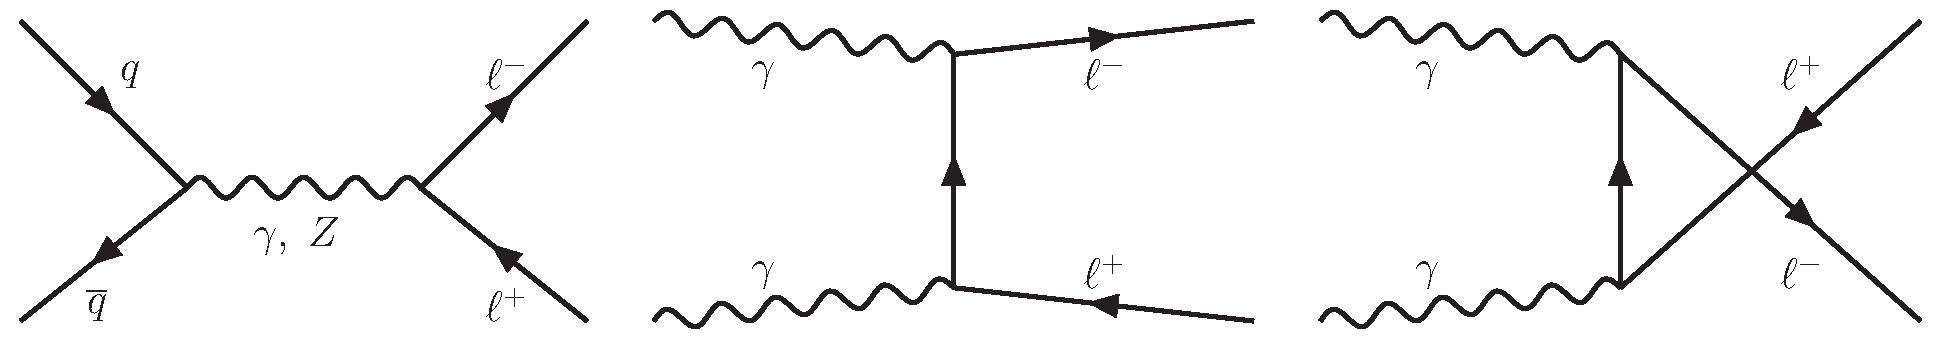
\includegraphics[width=17cm]{figs/DYdiagrams.pdf}
    \end{center}
    \caption{Diagrams that contribute to lepton-pair production at
      hadron colliders at the Born level.}
\label{fig:photoninduced}
\end{figure}
%%%%%%%%%%%%%%%%%%%%%%%%%%%%%%%%%%%%%%%%%%%%%%%%%%%%%%%%%%%%%%%%

DIS structure functions and PDF evolution are computed with the {\tt
  APFEL} program~\cite{Bertone:2013vaa}, which is currently accurate
up to NNLO in pure QCD and NLO in QED, and includes the relevant mixed
QCD+QED corrections. This means that, on top of the pure QCD
contributions, the DGLAP evolution
equations~\cite{Gribov:1972ri,Dokshitzer:1977,Altarelli:1977zs} are
solved including the $\mathcal{O}\lp \alpha_s\alpha\rp$ and
$\mathcal{O}\lp \alpha^2\rp$ corrections to the splitting functions.

As far as the DIS structure functions are concerned, corrections of
$\mathcal{O}\lp \alpha\rp$ are also included which in turn lead to an
explicit dependence of the predictions on the photon PDF.  The details
on the implementation as well as a discussion on the impact of these
corrections are given in appendix~\ref{sec:appendixAPFEL}.

Heavy-quark (charm and bottom) mass effects to DIS structure functions
are taken into account using the FONLL-B(C) general-mass
scheme~\cite{Forte:2010ta} for the NLO (NNLO) fits.
%
As for the numerical values of the heavy-quark masses in the pole-mass
scheme, we take $m_c=1.47~$GeV and $m_b=4.5~$GeV as determined in \cite{Abramowicz:2015mha}, which is also 
consistent with the latest PDG averages~\cite{Agashe:2014kda}.
%
The reference values of the coupling constants are chosen to be
$\alpha_s(m_Z)=0.118$ and $\alpha(m_\tau=1.777\mbox{ GeV})=1/133.4$.

For the calculation of high-mass Drell-Yan cross sections, we use the
{\tt MadGraph5{\_}aMC@NLO}~\cite{Alwall:2014hca} program v2.4.3, which
includes the contribution from photon-initiated diagrams, interfaced
to {\tt APPLgrid}~\cite{Carli:2010rw} v1.4.7 through {\tt
  aMCfast}~\cite{amcfast} v1.3).
%
A tailored version of {\tt APPLgrid} is used, allowing to account for
the contribution of the photon-initiated processes \footnote{Modified version of APPLgrid available at: $https://github.com/scarrazza/applgridphoton$}.
%
The calculation is performed in the $n_f=5$ scheme neglecting mass
effects of charm and bottom quarks in the matrix elements, as
appropriate for a high-scale processes.

The kinematic phase-space coverage of the data is presented in Fig.~\ref{fig:data}.
%%%%%%%%%%%%%%%%%%%%%%%%%%%%%%%%%%%%%%%%%%%%%%%%%%%%%%%%%%%%%%%%                                                                  
\begin{figure}[t]
  \begin{center}
    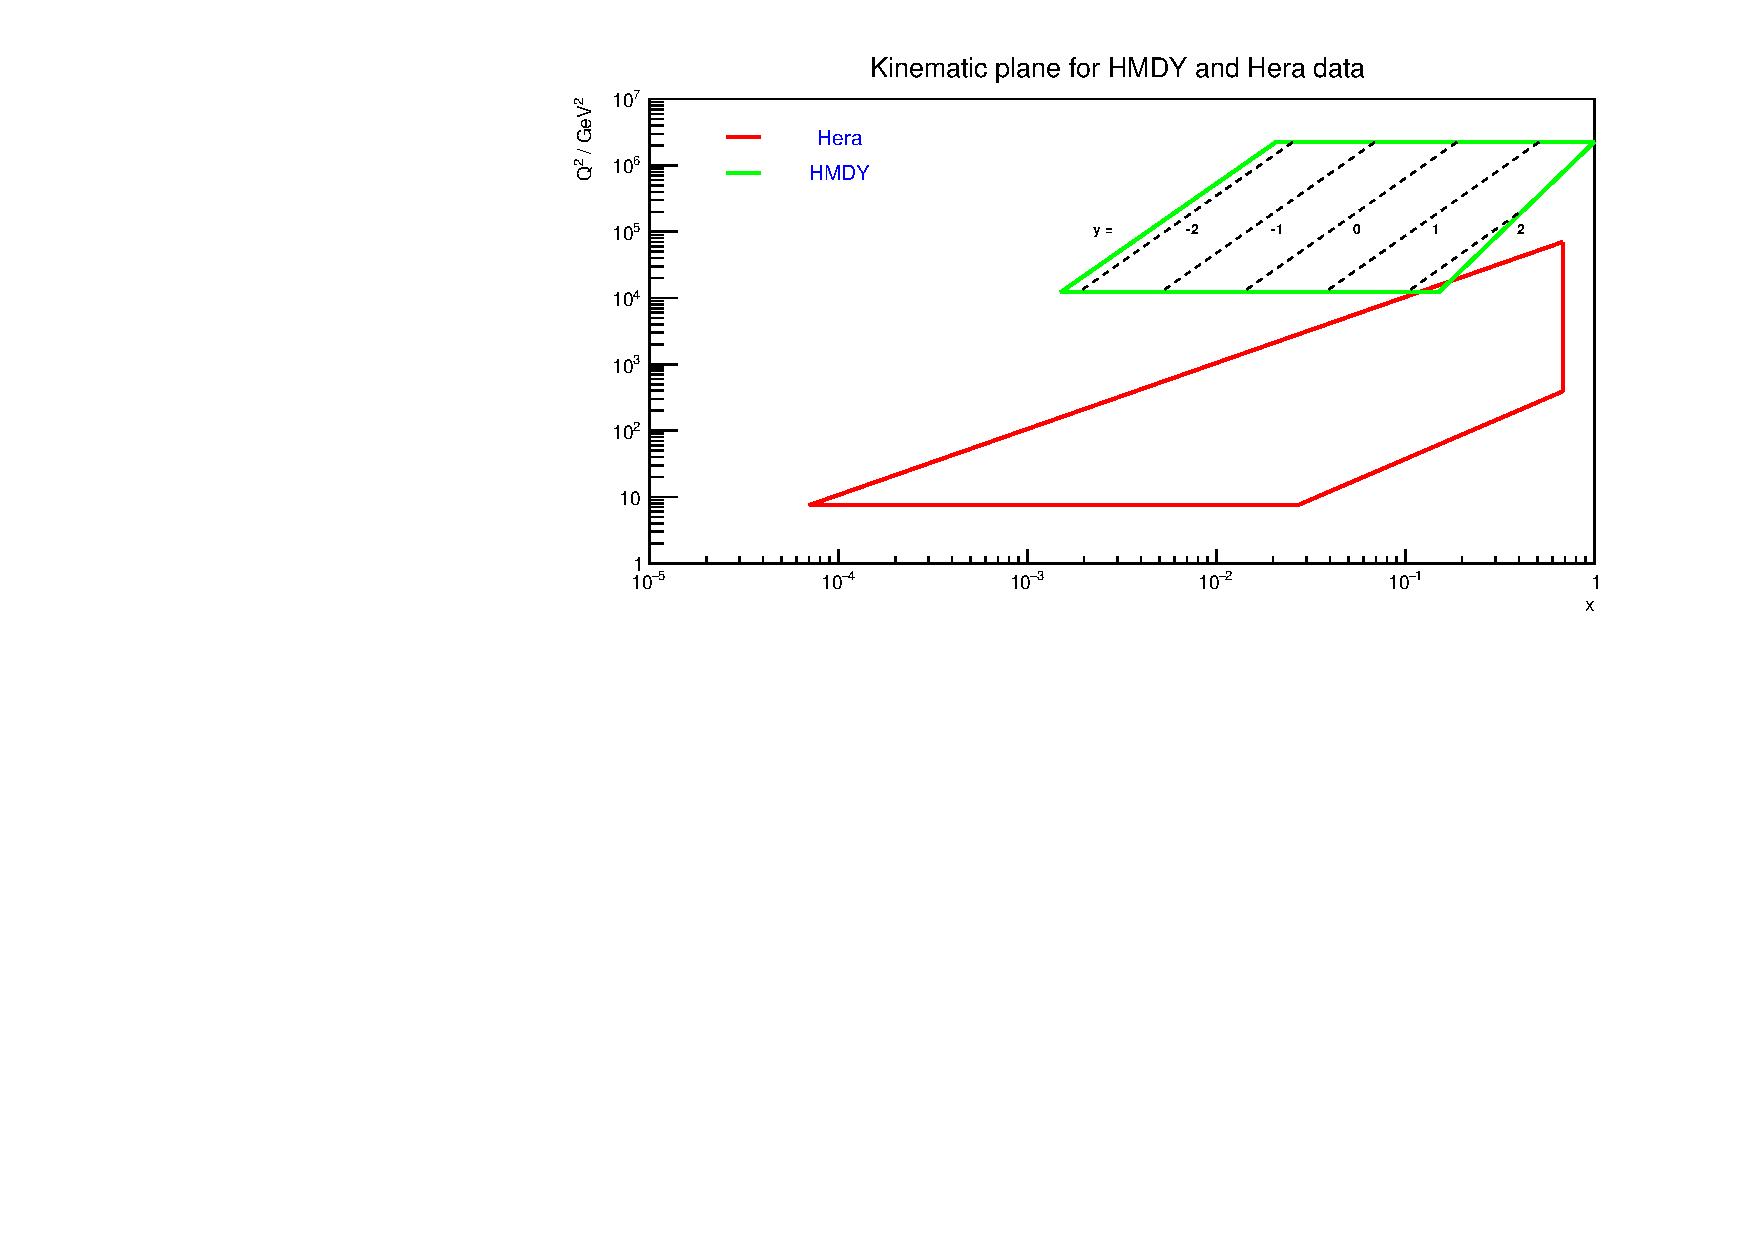
\includegraphics[width=10cm]{figs/kin2.pdf}
    \end{center}
    \caption{Kinematic coverage in $x$ and $Q^2$ plane of data used in this analysis: in red the HERA data, in green the high-mass DY data.}
\label{fig:data}
\end{figure}
%%%%%%%%%%%%%%%%%%%%%%%%%%%%%%%%%%%%%%%%%%%%%%%%%%%%%%%%%%%%%%%%      
The ATLAS high-mass Drell-Yan 8 TeV measurements include both the
single-differential (1D) invariant-mass distribution,
$d\sigma/dm_{ll}$, as well as the double-differential (2D)
distributions in $m_{ll}$ and $y_{ll}$,
$d^{2}\sigma/dm_{ll}d|y_{ll}|$, and in $m_{ll}$ and $\Delta\eta_{ll}$,
$d^{2}\sigma/dm_{ll}\Delta\eta_{ll}$.
%
For the invariant-mass distribution, there are 12 bins between 116 GeV
and 1.5 TeV; and for both of the double-differential distributions,
there are five different histograms, one for each of the different
invariant mass ranges, from the lowest bin with 116 GeV < $m_{ll}$ <
150 GeV to the highest bin with 500 GeV < $m_{ll}$ < 1500 GeV.
 %
The first three (last two) $m_{ll}$ bins are divided into 12 (6) bins
with fixed width, extending up to 2.4 and 3.0 for the $|y_{ll}^{mim}|$
and $|\Delta\eta_{ll}|$ distributions, respectively.
%
In Sect.~\ref{sec:results} we compare the impact on the photon PDF of
fitting either the 1D distributions or one of the two 2D
distributions.

In the theoretical calculations of the Drell-Yan cross section we use
dynamical renormalisation $\mu_{R}$ and factorisation $\mu_{R}$
scales, both set equal to the invariant mass $m_{ll}$ of the
respective bin.
%
The theoretical predictions for these measurements implement the
analysis cuts, including $m_{ll}\ge 116$ GeV, $\eta_l\le 2.5$,
$p_T^l \ge 40$ GeV$~(30)$ GeV for the leading (sub-leading) lepton.
%
The {\tt MadGraph5{\_}aMC@NLO} calculations used in this work were
benchmarked against the corresponding predictions (NLO QCD and LO QED,
including photon-induced processes) obtained with the {\tt FEWZ}
code~\cite{Gavin:2012sy} v3.1, finding agreement at the 1\% level or
better for both the 1D and the 2D distributions.
%
In order to achieve NNLO QCD and NLO EW accuracy in our theoretical
calculations, the NLO QCD + LO QED {\tt APPLgrid} tables generated
with {\tt aMCfast} have been supplemented by bin-by-bin $K$-factors,
defined as:
\begin{equation}
  \label{eq:kfactor}
  K \equiv\frac{\rm NNLO\  QCD  + NLO\  EW}{\rm NLO\  QCD + LO\  EW} \, ,
\end{equation}
using the MMHT2014 NNLO~\cite{Harland-Lang:2014zoa} PDF set both in
the numerator and in the denominator (NNLO $K$-factors depend very
mildly on the PDF set).
 %
The $K$-factors in Eq.~({\ref{eq:kfactor}) have been computed using
  the {\tt FEWZ} program, with the same settings as the corresponding
  NLO computations.
%

  In Fig.~\ref{fig:kf} we show the $K$-factors corresponding to the
  measurements included in our fits as a function of the dilepton
  rapidity $|y_{ll}|$, where each curve corresponds to a different
  dilepton invariant-mass $m_{ll}$ bin.
%
  We observe that the $K$-factors vary between 0.98 and 1.04,
  highlighting the fact that higher-order corrections to the Drell-Yan
  process are moderate, in particular at low values of $m_{ll}$ and in
  the central region.
%
  Even at forward rapidities, the $K$-factors modify the NLO result by
  at most 3\%.

%%%%%%%%%%%%%%%%%%%%%%%%%%%%%%%%%%%%%%%%%%%%%%%%%%%%%%%%
\begin{figure}[t]
\includegraphics[width=9cm]{figs/kf_2D.pdf}
\caption{The NNLO/NLO $K$-factors, defined in Eq.~(\ref{eq:kfactor}),
  that allow accounting for higher order QCD and EW effects in the PDF
  fits, as a function of the dilepton rapidity $|y_{ll}|$.  Each curve
  correspond to one of the $m_{ll}$ invariant mass bins.}
\label{fig:kf}
\end{figure}
%%%%%%%%%%%%%%%%%%%%%%%%%%%%%%%%%%%%%%%%%%%%%%%%%%%%%%%%

\section{Settings}
\label{sec:fitsettings}

In this section we discuss the settings of
the PDF fit, including the parametrization of the photon PDF
that will be adopted in the following.
%
The analysis will be carried out using the open-source
{\tt xFitter} framework~\cite{Alekhin:2014irh}.
%
The input evolution scale $Q_0$, where the PDFs
are parametrized, is taken to be $Q^2_0 = 7.5~$GeV$^2$.
%
This is also the value $Q^2_0=Q^2_{\rm min}$ used to set the
minimum value of $Q^2$ for those data points that enter the fit.
%
The charm PDF is generated perturbative from quarks and gluons
using the DGLAP equations, exploiting recent developments
in {\tt APFEL} which allow the use of displaced heavy quark
thresholds, so we use $\mu_c=Q_0 > m_c$.

The  expression for the $\chi^2$ used for the fit is the one
defined in Ref.~\cite{Aaron:2009aa}
%
Alternative forms have also been tried,
with no significant difference to our results.
% 
The PDF parametrisation input at $Q^2_0$ is determined by the technique of saturation of the $\chi^{2}$, namely one keeps increasing
the number of parameters until the $\chi^{2}$ does not improve further.
%
In this analysis,
the parametrised PDFs are the valence distributions $xu_{v}$ and $xd_{v}$, the gluon distribution $xg$, and the \textit{u}-type and \textit{d}-type sea quarks, $x\bar{U}$, $x\bar{D}$, where $x\bar{U} = x\bar{u}$ and $x\bar{D} = x\bar{d} + x\bar{s}$.
%
In addition, we also parametrize the photon distribution $x\gamma$.
%
The following  functional form will be used:
\begin{equation}
  \label{eq:parametrization}
xf(x) = Ax^{B}(1-x)^{C}(1+Dx+Ex^{2})
\end{equation}
where some of the normalisation parameters, in particular
$A_{u_{v}}$, $A_{d_{v}}$ and $A_{g}$, are constrained by the valence and momentum
sum rules.
%
The  parameters $B_{\bar{U}}$ and $B_{\bar{D}}$ are set equal to each other, such
the two quark sea distributions share a common small-$x$ behaviour.
%
Since the measurements used here are not sensitive to the 
strangeness content of the proton, we fix $x\bar{s} = 0.5x\bar{D}$, consistent with
the ATLAS 
analysis of inclusive $W$ and $Z$ production~\cite{Aad:2012sb}.
%
A further constraint $A_{\bar{U}} = 0.5 A_{\bar{D}}$ is imposed such that $x\bar{u} \to x\bar{d}$ as $x \to 0$.
The \textit{D} and \textit{E} parameters are added one by one
to the parametrization Eq.~(\ref{eq:parametrization}) until no significant 
improvement in $\chi^{2}$ is found. 

Following this method, the optimal parametrization found for this analysis turns
out to be the following for the quark and gluon PDFs:
\begin{eqnarray}
  \nonumber
  xu_v(x) &&= A_{u_v}x^{B_{u_v}}(1-x)^{C_{u_v}}(1+E_{u_v}x^{2})\, , \\
  \nonumber
xd_v(x) &&= A_{d_v}x^{B_{d_v}}(1-x)^{C_{d_v}}\, , \\
x\bar{U}(x) &&= A_{\bar{U}}x^{B_{\bar{U}}}(1-x)^{C_{\bar{U}}}\, , \\
\nonumber
x\bar{D}(x) &&= A_{\bar{D}}x^{B_{\bar{D}}}(1-x)^{C_{\bar{D}}}\, , \\
\nonumber
\label{eq:param}
xg(x) &&= A_{g}x^{B_{g}}(1-x)^{C_{g}}(1+E_{g}x^{2})\, ,
\end{eqnarray}
while for the photon PDF instead we use
\begin{equation}
x\gamma(x) = A_{\gamma}x^{B_{\gamma}}(1-x)^{C_{\gamma}}(1+D_{\gamma}x+E_{\gamma}x^{2}) \, .
\end{equation}
Note that now the photon PDF also enters the momentum sum rule.

The parametrisation of the quark and gluon PDFs Eq.~(\ref{eq:param}) differs from the one used
in the HERAPDF2.0 analysis in various aspects.
%
First of all, we use a higher value of the input evolution scale $Q^2_0$, which is helpful
to stabilize the fit of the photon PDF.
%
Second, the additional negative term in the parametrization of the gluon
is not required here, since we use a more stringent cut $Q_{\rm min}^2$ which removes
some of the low-$x$ data (since they do not provide any information on the photon).
%
Third, the results of the parametrization scan are different due to the presence now
of the ATLAS high-mass Drell-Yan cross-section.

PDF uncertainties are estimated using the Monte Carlo
replica method~\cite{DelDebbio:2004xtd}, cross-checked
with the Hessian method~\cite{Pumplin:2001ct} using $\Delta\chi^2=1$.
%
The former is expected to be more robust than the latter, due to the potential
non-gaussian nature of the photon PDF uncertainties~\cite{Ball:2013hta}.
%
In addition, we have performed a number of cross-checks to assess the impact
of various model and parametrization uncertainties.
%
For the model uncertainties, we will consider variations of the charm mass
between $m_c=1.41$ GeV to 1.53 GeV; of the bottom mass between
$m_c=4.25$ GeV to 4.75 GeV; of the strong
coupling constant $\alpha_s(m_Z)$ between 0.116 to 0.120; as well
as of decreasing the strangeness fraction down to  $f_s=0.4$.
%
Concerning the parametrization uncertainties, we will quantify the impact of
 increasing the input parametrization scale
 (and minimum $Q^2$ cut) up to $Q_0^2=Q^2_{\rm min}=10$ GeV$^2$, as well as
 of additional parameters in Eq.~(\ref{eq:param}) that make little difference to the $\chi^2$ of the fit, but which can change the shape of the PDFs, in particular the extra negative term for the gluon; $D_{u_v}$, $D_{\bar{u}}$ and $E_{\bar{d}}$.

\section{Results}

\subsection{Sensitivity}
 show impact of HM DY on PDFs using sensitivity studies based on
pseudo-data, for which we only use the data uncertainties, while central 
value are fixed:
 HERA I+II vs HERA I+II + HMDY --> see the sensitivity plots from the previous email


conclusion: HMDY data has a large impact on photonPDF 



\subsection{PDF Fits}

In order to make a full PDF fit the  ATLAS Drell-Yan data data are fitted together with the final combined inclusive 
cross section data from HERA~\cite{hera}. The HERA data provide information on the quark/antiquark and gluon content of 
the proton and the Drell-Yan data add information on the photon content of the proton. {\it and maybe refine the quark/antiquark content, refer sensitivity study}.   
The NLO and NNLO pQCD predictions are fitted to the data using the xFitter open source pQCD fitting platform~\cite{xFitter}.
The DGLAP equations~\cite{dglap} are solved using the programme QCDNUM which has been modified to include 
the photon PDF in the proton~\cite{qcdnum}.
The DGLAP equations yield the PDFs at all scales if they are input as finctions of $x$ at a starting scale $Q^2_0$, which 
should be large enough that perturbative QCD can be assumed to be valid. For the present analysis this value is chosen
to be $Q^2_0 = 7.5~$GeV$^2$. This is also the value chosen for the minimum value of $Q^2$ for data entering the fit.
The charm and beauty masses are chosen to be $m_c=1.47~$GeV and $m_b=4.5~$GeV following the HERA analysis. 
The value of $\alpha_s(M_Z)$ is chosen to be $\alpha_s(M_Z)=0.118$~\cite{PDG}. 
The value of $Q^2_0$ is above the charm mass squared, however a version of the programme 
is used which displaces the charm threshold from the charm mass~\cite{charmthresh} such that the threshold is at $Q^2_0$.
The form of the $\chi^2$ used for the fit is that defined in the H1 paper~\cite{h1chisqdef}. 
Alternative forms have also been tried with no significant difference to our results.
 
The PDF parametrisation input at $Q^2_0$ is determined by the technique of saturation of the $\chi^{2}$~\cite{h1chisqsat}.
The parametrised PDFs are the valence distributions $xu_{v}$ and $xd_{v}$, the gluon distribution $xg$, and the \textit{u}-type and \textit{d}-type sea, $x\bar{U}$, $x\bar{D}$, where $x\bar{U} = x\bar{u}$ and $x\bar{D} = x\bar{d} + x\bar{s}$, and finally the photon distribution $x\gamma$. The following standard functional form is used to parametrise them:
\begin{equation}
xf(x) = Ax^{B}(1-x)^{C}(1+Dx+Ex^{2})
\end{equation}
where the normalisation parameters $A_{u_{v}}$, $A_{d_{v}}$ and $A_{g}$ are constrained by the number sum-rules and the 
momentum sum-rule, respectively. The \textit{B} parameters $B_{\bar{U}}$ and $B_{\bar{D}}$ are set equal, such that there 
is a single \textit{B} parameter for the sea distribution. The data are not sensitive to the 
strangeness content of the proton which is thus set such that $x\bar{s} = 0.5\bar{D}$, following the ATLAS 
analysis~\cite{atlasstrange}. The further constraint $A_{\bar{U}} = 0.5 A_{\bar{D}}$ is imposed such that $\bar{u}=x\bar{d}$ as $x \to 0$.
The \textit{D} and \textit{E} parameters are introduced one by one until no significant 
improvement in $\chi^{2}$ is found. 

 For the NLO fit a $\chi^{2}/ndf = 1225.3/1084 = 1.13$, with a partial $\chi^2/ndp = 46.9/48$ for the high-mass Drell-yan data [{\it please separate contribution of log term and correlated term in the partial chisq table to allow this calculation to be accurate- I estimated it}], is achieved for the following parametrisation, which has 15 parameters for the quarks and gluons and 5 parameters for the photon:
\begin{eqnarray}
xu_v(x) = A_{u_v}x^{B_{u_v}}(1-x)^{C_{u_v}}(1+D_{u_v}x+E_{u_v}x^{2}), \\
xd_v(x) = A_{d_v}x^{B_{d_v}}(1-x)^{C_{d_v}}, \\
x\bar{U}(x) = A_{\bar{U}}x^{B_{\bar{U}}}(1-x)^{C_{\bar{U}}}(1+D_{\bar{U}}x+E_{\bar{U}}x^2), \\
x\bar{D}(x) = A_{\bar{D}}x^{B_{\bar{D}}}(1-x)^{C_{\bar{D}}}, \\
xg(x) = A_{g}x^{B_{g}}(1-x)^{C_{g}}(1+E_{g}x^{2}), \\
x\gamma(x) = A_{\gamma}x^{B_{\gamma}}(1-x)^{C_{\gamma}}(1+D_{\gamma}x+E_{\gamma}x^{2}) \\
\end{eqnarray}
Figures **%Fig.~\ref{PDF_100GeV}
 show the PDF distributions $x_{u_v},xd_{d_v},x\bar{u}, x\bar{d}, xg$ at $Q^{2}$ = 10$^{2}$ GeV$^{2}$, while  Figures **%Fig.~\ref{PDF_1000GeV} 
show them at $Q^{2}$ = 10$^{4}$ GeV$^{2}$. {\it Redo figures for the just Dubar final parametrisation, conisder adding +Dg and Eubar as parametrisation variations. Also consider model variations  like change of Q2cut, Q20, fs, mc,mb}.
[{\it When showing PDF distributions for the NLO fit at two scales.
show ubar and dbar as well, sbar,cbar,bbar are not interesting in the current context.
Then repeat with this parametrisation at NNLO and quote NNLO partial chisq for DY data. Make plots of NNLo vs NLo only for the photon PDF. 
Here you will almost 
certainly find a worse overall chisq, but it will be worse for HERA which really likes the 
negative gluon term. It will probably not be worse for the DY. We do not need to discuss the HERA NNLO features here}].
%\begin{figure}
%\includegraphics[width=5.14cm]{uv_100.ps} 
%\includegraphics[width=5.14cm]{dv_100.ps} 
%\includegraphics[width=5.14cm]{g_100.ps} 
%\caption{PDF distributions at $Q^{2}$ = 10$^{2}$ GeV$^{2}$: (a) \textit{u} - valence; (b) \textit{d} - valence; (c) gluon}
%\label{PDF_100GeV}
%\end{figure}
%\begin{figure}
%\centering
%\includegraphics[width=5.14cm]{uv_1000}
%\includegraphics[width=5.14cm]{dv_1000} 
%\includegraphics[width=5.14cm]{g_1000} 
%\caption{PDF distributions at $Q^{2}$ = 10$^{4}$ GeV$^{2}$: (a) \textit{u} - valence; (b) \textit{d} - valence; (c) gluon}
%\label{PDF_1000GeV}
%\end{figure}
In these figures comparisons are made to the NNPDF3.0PDF set [{\it use NNPDF3.0 not the rwg version}] and the HERAPDF2.0 set.
One can see that the shape of the $xd_{u_v}$ distribution is close to that of HERAPDF2.0 
because of the dominance of HERA data in the fit. {\it More comments?}

%Fig.~\ref{hmDY_2D} 
Fig. shows the comparison between the hmDY two-dimensional distribution and the predictions. {\it Just make it for the 15 parameter Dubar fit.}
%\begin{figure}
%\centering
%\subfigure[]{\includegraphics[width=5.14cm]{picture_confirmation/hmDY_1}} 
%\subfigure[]{\includegraphics[width=5.14cm]{picture_confirmation/hmDY_2}} 
%\subfigure[]{\includegraphics[width=5.14cm]{picture_confirmation/hmDY_3}} 
%\subfigure[]{\includegraphics[width=5.14cm]{picture_confirmation/hmDY_4}} 
%\subfigure[]{\includegraphics[width=5.14cm]{picture_confirmation/hmDY_5}} 
%\caption{Comparison between $\dfrac{d^{2}\sigma}{dm_{ll}d|y_{ll}|}$ hmDY data and fit results; the various fit differ just on the number of free parameters.}
%\label{hmDY_2D}
%\end{figure}
The $\chi^{2}$ values for each separate fitted dataset and the output parameters from the various fits can be found in Tables * %Fig.~\ref{chi2_scan} 
and in Table *%Fig.~\ref{par_scan} 
respectively. {\it Do this ONLy for the central +Dubar fit}
%\begin{figure}
%\centering
%\subfigure[]{\includegraphics[width=8.44cm]{picture_confirmation/chi2_scan}} 
%\caption{Comparison between $\chi^{2}$ for the different fits just described above.}
%\label{chi2_scan}
%\end{figure}
%\begin{figure}
%\centering
%\subfigure[]{\includegraphics[width=12.14cm]{picture_confirmation/par_scan}} 
%\caption{Comparison between the output parameters of the different fits just described above.}
%\label{par_scan}
%\end{figure}

Focusing now on the photon PDF distribution, there is some impact on the photon PDF from adding parameters to the quark and gluon PDFS, particularly from adding a $D_g$ and an $E_{\bar{U}}$ parameter.
This impact has been included in the parametrisation variations and is shown 
both at the starting scale (7.5 GeV$^{2}$) and at 10$^{4}$ GeV$^{2}$ 
 in Fig *
%Fig.~\ref{photon_scan}. 
%\begin{figure}
%\centering
%\subfigure[]{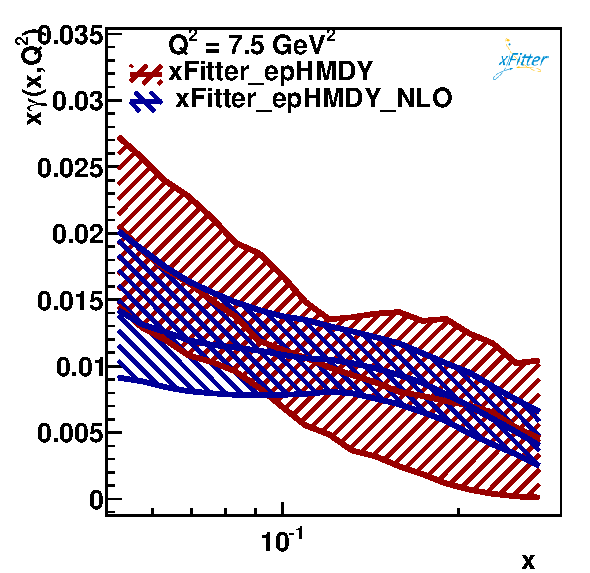
\includegraphics[width=6.96cm]{picture_confirmation/photon_7_5}} 
%\subfigure[]{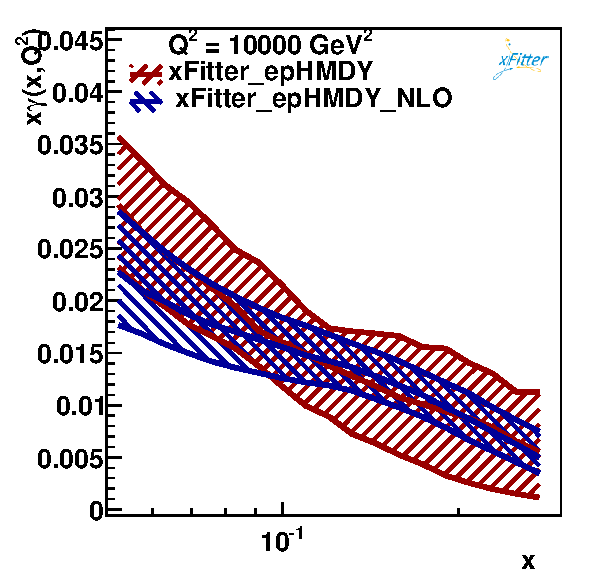
\includegraphics[width=6.96cm]{picture_confirmation/photon_10000}} 
%\caption{Comparison between the photon PDF distributions for the different fits just described above: (a) at the starting scale; (b) at the evolved scale.}
%\label{photon_scan}
%\end{figure}

Fig %Fig.~\ref{photon_zoom} 
shows the photon distribution in the range $0.045 < x < 0.35$, region where high mass DY data are most 
sensitive to this quantity. The new fit results 
have an uncertainty between 20{\%} and 30{\%}, which is 
considerably reduced compared to the  NNPDF30qed NLO photon PDF which is also 
shown for comparison. {\it Not the rwg version}.
The predictions for the LUXqed~\cite{luxqed} photon PDF and the 
HKR photon PDF~\cite{hkr}  are shown compared to the NNLO PDF from the present analysis in Fig.** {\it Compare our NNLO PDF when you have it}.
In this kinematic region, the fit
 predictions agree with LUXqed and with the HKR photon PDF at the 1-$\sigma$ level. 


%\begin{figure}
%\centering
%\subfigure[]{\includegraphics[width=6.96cm]{picture_confirmation/photon_7_5_zoom}} 
%\subfigure[]{\includegraphics[width=6.96cm]{picture_confirmation/photon_10000_zoom}} 
%\caption{Comparison between the photon PDF distributions for the different fits just described above: (a) at the starting scale; (b) at the evolved scale.}
%\label{photon_zoom}
%\end{figure}



%\begin{figure*}[th]
%\begin{centering}
%\includegraphics[width=0.75\textwidth]{figs/}
%\par\end{centering}
%\caption{alphas across bottom transition }
%\end{figure*}


\section{Conclusions}

\label{sec:conclusions}

The determination of the photon content of the proton has
attracted a considerable amount of attention recently.
%
In this work, we have presented a determination of the photon PDF from
a PDF fit based on HERA inclusive structure functions and recent ATLAS measurements
of high-mass Drell-Yan cross-sections.
%
We confirm that the high-mass DY data provides significant constraints on the photon PDF
in the region $0.05 \le x \le 0.3$.
%
We find good agreement within uncertainties with two recent calculations of the photon PDF,
LUXqed and HKR for the region of $x$ where the DY data has sensitivity.
%
On the other hand, we also find that a direct determination of the photon PDF
is still far from being competitive with the LUXqed calculation, which uses as input
the high-precision measurements of inclusive structure function of the proton.

The results of this study have been made possible by a number of technical developments
that should be of direct application for future PDF fits accounting for QED corrections,
such as the implementation of $\mathcal{O}\lp alpha^2\rp$ corrections to the DGLAP
evolution and the DIS coefficient functions in {\tt APFEL} or the extension of
{\tt aMCfast} to be able to deal with the photon-initiated calculations provided
by {\tt MadGraph5\_aMC@NLO}.
%
Our results also illustrate the flexibility of the {\tt xFitter} toolbox to extend
its capabilities from the standard quark and gluon PDF fits.


{\bf Acknowledgements}.
%
We thank L. Harland-Lang for providing us a {\tt LHAPDF6} grid
of the HKR photon determination.
%
The work of V.~B., F.~G. and J.~R. has been supported
by the European Research Council Starting Grant ``PDF4BSM".




\appendix

\section{NLO QED corrections in APFEL} \label{sec:appendixAPFEL}

In this appendix we present the details of the implementation of the
joint NLO QCD+QED corrections in {\tt APFEL}.
%
As discussed in~\cite{Bertone:2013vaa},
the implementation of LO
QED effects presents many simplifications,
in particular the fact that QED and QCD
corrections do not mix, and therefore the DGLAP evolution
equations as well as the
$\alpha_s$ and $\alpha$ running are decoupled.
%
On the other hand,
when going
to NLO this property does not
hold anymore,
and there QED and QCD contributions mix both in the DGLAP and in the
coupling evolution equations.
%
On top of this complication, these mixed corrections induce
the presence of diagrams in which a real photon is present either in
the initial or in the final state and that have to be included in the
computation of the DIS structure functions.

In the following we will
first discuss how to generalize the coupling evolution equations
(finding that the presence of the mixed QCD+QED terms leads to a
negligible difference in the running), we will then turn to the DGLAP,
and finally we will consider both neutral-current and charged-current
DIS structure functions.

\subsection{Evolution of the couplings}

As  mentioned above, NLO QCD+QED corrections induce the presence of
mixed terms at the level of the running of the
corresponding coupling constants.
%
That is,
the QCD $\beta$-function receives corrections proportional to $\alpha$
and, vice-versa, the QED $\beta$-function receives corrections
proportional to $\alpha_s$, in such a way that the coupling evolution
equations read:
\begin{equation}\label{CoupledEq}
\begin{array}{rcl}
\displaystyle \mu^2\frac{\partial \alpha_s}{\partial \mu^2} &=& \displaystyle
                                                \beta^{\rm QCD}(\alpha_s,\alpha)\,,\\
\\
\displaystyle \mu^2\frac{\partial \alpha}{\partial \mu^2} &=& \displaystyle \beta^{\rm QED}(\alpha_s,\alpha)\,.
\end{array}
\end{equation}
As a consequence, these evolution equations form a set of coupled
differential equations. Up to three loops ($i.e.$ NLO), the
$\beta$-functions can be expanded as:
\begin{equation}
\beta^{\rm QCD}(\alpha_s,\alpha) = -\alpha_s\left[\beta_0^{(\alpha_s)}\left(\frac{\alpha_s}{4\pi}\right)+\beta_1^{(\alpha_s\alpha)}\left(\frac{\alpha_s}{4\pi}\right) \left(\frac{\alpha}{4\pi}\right)+\beta_1^{(\alpha_s^2)}\left(\frac{\alpha_s}{4\pi}\right)^2+\dots\right]\,,
\end{equation}
and:
\begin{equation}
\beta^{\rm QED}(\alpha_s,\alpha) = -\alpha\left[\beta_0^{(\alpha)}\left(\frac{\alpha}{4\pi}\right)+\beta_1^{(\alpha\alpha_s)}\left(\frac{\alpha}{4\pi}\right) \left(\frac{\alpha_s}{4\pi}\right)+\beta_1^{(\alpha^2)}\left(\frac{\alpha}{4\pi}\right)^2+\dots\right]\,,
\end{equation}
where the ``new'' terms are the mixing terms
$\beta_1^{(\alpha_s\alpha)}$ and $\beta_1^{(\alpha\alpha_s)}$, and the
pure NLO QED term $\beta_1^{(\alpha^2)}$ have been computed in
Ref.~\cite{Surguladze:1996hx}. Taking into account a factor four due
the different definitions of the expansion parameter and writing
explicitly the color factors one finds:
\begin{equation}\label{eq:NewBetaTerms}
\beta_1^{(\alpha_s\alpha)} = -2\sum_{i=1}^{n_f}
e_q^2\,\qquad\beta_1^{(\alpha\alpha_s)} = -\frac{16}{3}N_c\sum_{i=1}^{n_f} e_q^2\,,\qquad \beta_1^{(\alpha^2)} = -4\left(n_l+N_c\sum_{i=1}^{n_f} e_q^2\right)\,.
\end{equation}
where $N_c=3$ is the number of colors, $e_q$ is the electric charge of
the quark flavour $q$, and $n_f$ and $n_l$ are the numbers of active
quark and leptons flavours, respectively.


Eq.~(\ref{CoupledEq}) can be written in the vectorial form:
\begin{equation}\label{CoupledEqVect}
\mu^2\frac{\partial {\bm \alpha}}{\partial \mu^2} = {\bm \beta}\left({\bm \alpha}(\mu)\right)\,,
\end{equation}
with:
\begin{equation}
  {\bm \alpha} = {\alpha_s \choose \alpha}\qquad\mbox{and}\qquad  {\bm \beta} = {\beta^{\rm QCD} \choose \beta^{\rm QED}}\,.
\end{equation}
Eq.~(\ref{CoupledEqVect}) is an ordinary differential equation that
can be numerically solved using the Runge-Kutta method.

The first two terms in eq.~(\ref{eq:NewBetaTerms}) are responsible for
the coupling of the evolution of $\alpha_s$ and $\alpha$ and thus they
introduce a complication that affects both the implementation and the
performance of the relative code. One can then ask what is the effect
of their presence and whether their removal makes a substantial
difference. In Fig.~\ref{fig:CouplingEvol} we show the comparison
between the evolution at NLO of both couplings $\alpha_s$ and $\alpha$
including and excluding the mixing terms in the respective
$\beta$-functions. The evolution is performed between the $Z$ mass
scale $M_Z$ and 10 TeV with 5 active quark flavours and 3 active
lepton flavours and uses as boundary conditions
$\alpha_s(M_Z) = 0.118$ and $\alpha(M_Z) = 1/128$. The two curves in
Fig.~\ref{fig:CouplingEvol} are normalised to the respective curve
without mixing terms. It is clear that the mixed terms lead to tiny
relative differences that are at most of $\mathcal{O}(10^{-4})$ at 10
TeV for $\alpha_s$ and $\mathcal{O}(10^{-3})$ at the same scale for
$\alpha$. We conclude that the mixed terms in the $\beta$-functions
have a negligible effect on the coupling evolution and thus we exclude
them to make the code simpler and improve the performance without
introducing any significant inaccuracy.

%%%%%%%%%%%%%%%%%%%%%%%%%%%%%%%%%%%%%%%%%%%%%%%%%%%%%%%%
\begin{figure}[h]
\includegraphics[width=6cm,angle=270]{figs/couplings.eps} 
\caption{Comparison between the running with the scale
$Q$ of the QCD and QED couplings,
  $\alpha_s$ and $\alpha$, including or not the mixed terms in
  the corresponding $\beta$-functions.
%
The curves are normalised to the result of the respective coupling
  running without the mixing terms.}
\label{fig:CouplingEvol}
\end{figure}
%%%%%%%%%%%%%%%%%%%%%%%%%%%%%%%%%%%%%%%%%%%%%%%%%%%%%%%%

\subsection{Impact on PDF evolution}

Next, we address the question of implementing the full NLO
QCD+QED corrections to the DGLAP evolution equations. Here we limit
ourselves to consider only the photon PDF without including the
leptons. The generalisation to the full set of PDFs can be achieved
relatively easily following the same steps discussed below.

The first step towards an efficient implementation of the solution of
the DGLAP equations in the presence of QED corrections is the adoption
of a suitable set of combinations of PDFs that diagonalize the
splitting function matrix, decoupling as many DGLAP equations as
possible. Such a set of combinations (or basis) was already introduced
in Appendix A of Ref.~\cite{Bertone:2015lqa} and will be used also
here (without considering the distributions involving leptons). The
basis reads:
\begin{equation}\label{eq:EvolBasis}
\begin{array}{ll}
\mbox{\texttt{ 1} : }g & \\
\mbox{\texttt{ 2} : }\gamma & \\
\mbox{\texttt{ 3} : }\displaystyle \Sigma = \Sigma_u + \Sigma_d & \quad
\mbox{\texttt{9} : }\displaystyle V =V_u +  V_d\\
\mbox{\texttt{ 4} : } \displaystyle \Delta_\Sigma = \Sigma_u - \Sigma_d& \quad\displaystyle 
\mbox{\texttt{10} : } \Delta_V = V_u - V_d\\
\mbox{\texttt{ 5} : }T_1^u = u^+ - c^+ &\quad \mbox{\texttt{11} : }V_1^u = u^- - c^- \\
\mbox{\texttt{ 6} : }T_2^u = u^+ + c^+ - 2t^+ &\quad \mbox{\texttt{12} : }V_2^u = u^- + c^- - 2t^-\\
\mbox{\texttt{ 7} : }T_1^d = d^+ - s^+ &\quad \mbox{\texttt{13} : }V_1^d = d^- - s^- \\
\mbox{\texttt{ 8} : }T_2^d = d^+ + s^+ - 2b^+ &\quad \mbox{\texttt{14}
                                               : }V_2^d = d^- + s^- -
                                               2b^-\\
\end{array}
\end{equation}
where we have defined $q^\pm = q\pm\overline{q}$ with
$q = u,d,s,c,b,t$ and:
\begin{equation}
\begin{array}{ll}
\Sigma_u = u^++c^++t^+, &\quad V_u = u^-+c^-+t^-,\\
\\
\Sigma_d = d^++s^++b^+,&\quad V_d = d^-+s^-+b^-\,.
\end{array}
\end{equation}
The second step is construct the splitting function matrix responsible
for the evolution of each one of the distributions defined above. To
do so, we split each splitting function $P$ into a pure QCD term
$\widetilde{P}$, which only depends on $\alpha_s$, and a QCD+QED
correction term $\bar{P}$, which instead contains contributions having
at least one power of $\alpha$ but that can also contain mixed
terms. In practice:
\begin{equation}
P = \widetilde{P} + \bar{P}\,,
\end{equation}
where:
\begin{equation}\label{eq:PureQCDSplittings}
\widetilde{P} = \alpha_s \mathcal{P}^{(1,0)} + \alpha_s^2 \mathcal{P}^{(2,0)}+\dots\,,
\end{equation}
and:
\begin{equation}\label{eq:QCD+QEDSplittings}
\bar{P} = \alpha \mathcal{P}^{(0,1)} + \alpha_s\alpha \mathcal{P}^{(1,1)}+\alpha^2 \mathcal{P}^{(0,2)}\dots
\end{equation}
Note that in the r.h.s. of both eqs.~(\ref{eq:PureQCDSplittings})
and~(\ref{eq:QCD+QEDSplittings}) we are using the notation of
Refs.~\cite{deFlorian:2015ujt,deFlorian:2016gvk} to indicate the power
of $\alpha_s$ and $\alpha$ that a given splitting function multiplies.

The structure of the pure QCD splitting function matrix
$\widetilde{P}$ as well as the first term in $\bar{P}$, which
represents the LO QED correction, in the basis given in
eq.~(\ref{eq:EvolBasis}) was discussed in
Ref.~\cite{Bertone:2015lqa}. It is now necessary to analyze the
structure of the two additional terms $\mathcal{P}^{(1,1)}$ and
$\mathcal{P}^{(0,2)}$. Let us start we the
$\mathcal{O}(\alpha_s\alpha)$ correction. The resulting evolution
equations at this order are:
\begin{equation}
\begin{array}{rcl}
\displaystyle\left.\mu^2\frac{\partial}{\partial \mu^2}
\begin{pmatrix}
g\\
\gamma\\
\Sigma\\
\Delta_\Sigma
\end{pmatrix}
\right|_{\mathcal{O}(\alpha_s \alpha)} &=& \displaystyle \begin{pmatrix}
e_\Sigma^2 \mathcal{P}^{(1,1)}_{gg}      & e_\Sigma^2 \mathcal{P}^{(1,1)}_{g\gamma} & \eta^+\mathcal{P}^{(1,1)}_{gq} & \eta^-\mathcal{P}^{(1,1)}_{gq} \\
e_\Sigma^2 \mathcal{P}^{(1,1)}_{\gamma g} & e_\Sigma^2 \mathcal{P}^{(1,1)}_{\gamma\gamma} & \eta^+\mathcal{P}^{(1,1)}_{\gamma q} &\eta^-\mathcal{P}^{(1,1)}_{\gamma q} \\
2 e_\Sigma^2 \mathcal{P}^{(1,1)}_{qg}    & 2 e_\Sigma^2 \mathcal{P}^{(1,1)}_{q\gamma} & \eta^+\mathcal{P}^{+(1,1)}  & \eta^-\mathcal{P}^{+(1,1)}\\
2 \delta_e^2 \mathcal{P}^{(1,1)}_{qg} & 2 \delta_e^2 \mathcal{P}^{(1,1)}_{q\gamma} &\eta^-\mathcal{P}^{+(1,1)} &\eta^+\mathcal{P}^{+(1,1)}
\end{pmatrix}\otimes
\begin{pmatrix}
g\\
\gamma\\
\Sigma\\
\Delta_\Sigma
\end{pmatrix}
\end{array}\,,
\end{equation}

\begin{equation}
\displaystyle\left.\mu^2\frac{\partial}{\partial \mu^2}
\begin{pmatrix}
V\\
\Delta_V
\end{pmatrix} \right|_{\mathcal{O}(\alpha_s \alpha)}= 
\begin{pmatrix}
\eta^+\mathcal{P}^{-(1,1)} & \eta^-\mathcal{P}^{-(1,1)} \\
\eta^-\mathcal{P}^{-(1,1)} & \eta^+\mathcal{P}^{-(1,1)} 
\end{pmatrix}\otimes
\begin{pmatrix}
V\\
\Delta_V
\end{pmatrix}\,,
\end{equation}

\begin{equation}
\begin{array}{ll}
\begin{array}{rcl}
\displaystyle \left.\mu^2\frac{\partial T^u_{1,2}}{\partial \mu^2}\right|_{\mathcal{O}(\alpha_s \alpha)} &=&
\displaystyle e_u^2\mathcal{P}^{+(1,1)}\otimes T^u_{1,2}
\end{array}\,, &
\begin{array}{rcl}
\displaystyle \left.\mu^2\frac{\partial T^d_{1,2}}{\partial \mu^2}\right|_{\mathcal{O}(\alpha_s \alpha)} &=&
\displaystyle e_d^2\mathcal{P}^{+(1,1)} \otimes T^d_{1,2}
\end{array}\,,
\\
\\
\begin{array}{rcl}
\displaystyle \left.\mu^2\frac{\partial V^u_{1,2}}{\partial \mu^2}\right|_{\mathcal{O}(\alpha_s \alpha)} &=&
\displaystyle e_u^2\mathcal{P}^{-(1,1)} \otimes V^u_{1,2}
\end{array}\,, &
\begin{array}{rcl}
\displaystyle \left.\mu^2\frac{\partial V^d_{1,2}}{\partial \mu^2}\right|_{\mathcal{O}(\alpha_s \alpha)} &=&
\displaystyle e_d^2\mathcal{P}^{-(1,1)}\otimes V^d_{1,2}
\end{array}\,.
\end{array}
\end{equation}
where $\otimes$ indicates the Mellin convolution and where we have
defined:
\begin{equation}
\begin{array}{rcl}
e_{\Sigma}^{2}& \equiv &\displaystyle
N_c(n_ue_{u}^{2}+n_de_{d}^{2})\,,\\
\\
\delta_e^2 & \equiv &\displaystyle N_c(n_u e_u^2 -n_d e_d^2)\,,\\
\\
\eta^{\pm} & \equiv & \displaystyle \frac{1}{2}\left(e_{u}^{2}\pm
  e_{d}^{2}\right)\,,\\
\end{array}
\end{equation}
with $e_u$ and $e_d$ the electric charges of the up- and down-type
quarks, and $n_u$ and $n_d$ the number of up- and down-type active
quark flavours (such that $n_u+n_d=n_f$).

Now we turn to consider the $\mathcal{O}(\alpha^2)$ corrections. The
explicit expressions of the splitting functions at this order are
reported in Ref.~\cite{deFlorian:2016gvk}. There are two main new
features that distinguish these expressions from the
$\mathcal{O}(\alpha)$ and $\mathcal{O}(\alpha_s\alpha)$ ones and that
are relevant to the implementation. The first is that, contrary to the
other cases in which the electric charges appeared to the second power
at the most, here they appear up to the fourth power. As a consequence
we need to introduce the new couplings:
\begin{equation}
\begin{array}{l}
+e_{\Sigma}^4 = N_c(n_{u} e_u^4 + n_{d} e_d^4)\,,\\
+\\
+\delta_e^4 = N_c(n_{u} e_u^4 - n_{d} e_d^4)\,.
\end{array}
\end{equation}

The second feature is that the dependence on the electric charges of
some of the $\mathcal{O}(\alpha^2)$ splitting functions is not
factorisable as it was the case for all the $\mathcal{O}(\alpha)$ and
$\mathcal{O}(\alpha_s\alpha)$ ones. In these cases we need to
distinguish between up-type and down-type splitting functions. After
some algebra we find that the $\mathcal{O}(\alpha^2)$ contributions to
the QCD+QED DGLAP equations read:

\begin{equation}
%\begin{array}{rcl}
\begin{array}{c}
\displaystyle\left.\mu^2\frac{\partial}{\partial \mu^2}
\begin{pmatrix}
g\\
\gamma\\
\Sigma\\
\Delta_\Sigma
\end{pmatrix}
  \right|_{\mathcal{O}(\alpha^2)} =\\
\\
 \displaystyle \frac12\begin{pmatrix}
    0 & 0 & 0 & 0 \\
    0 & 2e_\Sigma^4 \mathcal{P}_{\gamma\gamma}^{(0,2)} & e_u^4 \mathcal{P}_{\gamma
      u}^{(0,2)} + e_d^4 \mathcal{P}_{\gamma d} & e_u^4 \mathcal{P}_{\gamma u}^{(0,2)} - e_d^4 \mathcal{P}_{\gamma d}^{(0,2)}\\
    0 & 4 e_\Sigma^4 \mathcal{P}^{(0,2)}_{q\gamma} &
    e_u^4\mathcal{P}_{uu}^{+(0,2)}
    +e_d^4\mathcal{P}_{dd}^{+(0,2)}+2\eta^+e_\Sigma^2\mathcal{P}^{S(0,2)}_{qq} & e_u^4\mathcal{P}_{uu}^{+(0,2)}-e_d^4\mathcal{P}_{dd}^{+(0,2)} + 2\eta^-e_\Sigma^2\mathcal{P}^{S(0,2)}_{qq}\\
    0 & 4 \delta_e^4 \mathcal{P}^{(0,2)}_{q\gamma} & e_u^4\mathcal{P}_{uu}^{+(0,2)}
    -e_d^4\mathcal{P}_{dd}^{+(0,2)}+2\eta^-\delta_e^2
    \mathcal{P}^{S(0,2)}_{qq} & e_u^4\mathcal{P}_{uu}^{+(0,2)}+e_d^4\mathcal{P}_{dd}^{+(0,2)} + 2\eta^+\delta_e^2 \mathcal{P}^{S(0,2)}_{qq}
\end{pmatrix}\otimes
\begin{pmatrix}
g\\
\gamma\\
\Sigma\\
\Delta_\Sigma
\end{pmatrix}\,,
\end{array}
\end{equation}

\begin{equation}
\displaystyle\left.\mu^2\frac{\partial}{\partial \mu^2}
\begin{pmatrix}
V\\
\Delta_V
\end{pmatrix} \right|_{\mathcal{O}(\alpha^2)}= \frac12
\begin{pmatrix}
e_u^4\mathcal{P}_{uu}^{-(0,2)}+e_d^4\mathcal{P}_{dd}^{-(0,2)} & e_u^4\mathcal{P}_{uu}^{-(0,2)}-e_d^4\mathcal{P}_{dd}^{-(0,2)} \\
e_u^4\mathcal{P}_{uu}^{-(0,2)}-e_d^4\mathcal{P}_{dd}^{-(0,2)} & e_u^4\mathcal{P}_{uu}^{-(0,2)}+e_d^4\mathcal{P}_{dd}^{-(0,2)} 
\end{pmatrix}\otimes
\begin{pmatrix}
V\\
\Delta_V
\end{pmatrix}\,,
\end{equation}

\begin{equation}
\begin{array}{ll}
\begin{array}{rcl}
\displaystyle \left.\mu^2\frac{\partial T^u_{1,2}}{\partial \mu^2}\right|_{\mathcal{O}(\alpha^2)} &=&
\displaystyle e_u^4\mathcal{P}_{uu}^{+(0,2)}\otimes T^u_{1,2}
\end{array}\,, &
\begin{array}{rcl}
\displaystyle \left.\mu^2\frac{\partial T^d_{1,2}}{\partial \mu^2}\right|_{\mathcal{O}(\alpha^2)} &=&
\displaystyle e_d^4\mathcal{P}_{dd}^{+(0,2)} \otimes T^d_{1,2}
\end{array}\,,
\\
\\
\begin{array}{rcl}
\displaystyle \left.\mu^2\frac{\partial V^u_{1,2}}{\partial \mu^2}\right|_{\mathcal{O}(\alpha^2)} &=&
\displaystyle e_u^4\mathcal{P}_{uu}^{-(0,2)} \otimes V^u_{1,2}
\end{array}\,, &
\begin{array}{rcl}
\displaystyle \left.\mu^2\frac{\partial V^d_{1,2}}{\partial \mu^2}\right|_{\mathcal{O}(\alpha^2)} &=&
\displaystyle e_d^4\mathcal{P}_{dd}^{-(0,2)}\otimes V^d_{1,2}
\end{array}\,.
\end{array}
\end{equation}
It should be noticed that, as compared to the expressions presented in
Ref.~\cite{deFlorian:2016gvk}, we have factored out the electric
charges in such a way that the expressions of the splitting
functions are either independent from the electric charges or depend
only through the ratio $e_\Sigma^2/e_q^2$.

As an illustration, we study the effect of the
$\mathcal{O}(\alpha_s\alpha)$ and $\mathcal{O}(\alpha^2)$ corrections
to the DGLAP evolution equations on the $\gamma\gamma$ luminosity at
$\sqrt{s} = 13$ TeV, defined as:
\begin{equation}\label{eq:GammaGammaLumi}
\Phi_{\gamma\gamma}(M_X) = \frac1{s}\int_{M_X^2/s}^1
\frac{dx}{x} \gamma(x,M_X) \gamma\left(\frac{M_X^2}{xs},M_X\right)\,,
\end{equation}
as a function of the final state invariant mass $M_X$.

%%%%%%%%%%%%%%%%%%%%%%%%%%%%%%%%%%%%%%%%%%%%%%%%%%%%%%%%
\begin{figure}[t]
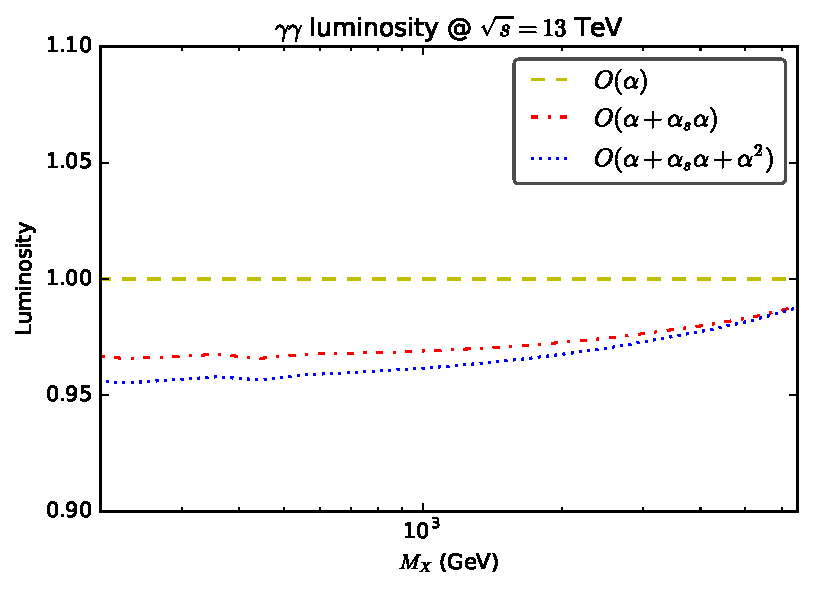
\includegraphics[width=8cm]{figs/lumi_13tev.pdf} 
\caption{The photon-photon
PDF luminosity $\mathcal{L}_{\gamma\gamma}$ at $\sqrt{s} = 13$ TeV as a
  function of the final state invariant mass $M_X$.
  %
  We compare the results of the photon evolved
  with only $\mathcal{O}(\alpha)$ corrections
  with the corresponding results with either
  $\mathcal{O}(\alpha+\alpha_s\alpha)$
  or $\mathcal{O}(\alpha+\alpha_s\alpha+\alpha^2)$ effects,
  normalized to the $\mathcal{O}(\alpha)$ result.
  %
  The calculation has been performed with
  NNPDF3.0QED as input.
}
\label{fig:GammaGammaLumi}
\end{figure}
%%%%%%%%%%%%%%%%%%%%%%%%%%%%%%%%%%%%%%%%%%%%%%%%%%%%%%%%

Fig.~\ref{fig:GammaGammaLumi} shows the behaviour of
$\Phi_{\gamma\gamma}$ computed using the photon PDF $\gamma$ of the
{\tt NNPDF30\_nlo\_as\_0118} PDF set evolved from $Q_0 = 1$ GeV to
$M_X$ including, on top of the pure QCD NLO evolution: only the LO QED
corrections $\mathcal{O}(\alpha)$ (yellow curve), also the mixed
corrections $\mathcal{O}(\alpha_s\alpha)$ (red curve), the full NLO
QCD+QED corrections, $i.e$
$\mathcal{O}(\alpha+\alpha_s\alpha+\alpha^2)$, (blue curve). All
predictions are normalized to the yellow curve. The
$\mathcal{O}(\alpha_s\alpha)$ and $\mathcal{O}(\alpha^2)$ corrections
have a small but non-negligible impact on the
$\gamma\gamma$-luminosity. In particular, these corrections suppress
$\Phi_{\gamma\gamma}$ by almost 5\% at relatively small values of
$M_X$, while the suppression gradually shrinks to 1-2\% as $M_X$
increases. As expected, most of the effect is ascribable to the
$\mathcal{O}(\alpha_s\alpha)$ corrections, while the
$\mathcal{O}(\alpha^2)$ ones have a substantially smaller impact.

\subsection{DIS structure functions}

When considering NLO QCD+QED corrections to the DIS structure
functions, one has to include into the hard cross sections all the
$\mathcal{O}(\alpha)$ diagrams where one photon is either in the
initial state or emitted from an incoming quark (or possibly an
incoming lepton). Such diagrams are of purely QED origin and no QCD
contributions are present. As a consequence, the corresponding
coefficient functions can easily be derived from the QCD expressions
just by properly adjusting the colour factors. In addition, this
correspondence holds regardless of whether mass effects are included
or not.

The main complication arises from the flavour structure. In fact, due
to the fact that the coupling of the photon is proportional to the
squared charge of the parton to which it couples (a quark or a
lepton), in the case of quarks the isospin symmetry is broken. In the
following we will address the case of Neutral-Current (NC), where
lepton and proton exchange a neutral boson $\gamma^*/Z$, and
Charged-Current (CC) structure functions separately, where instead
lepton and proton exchange a charged $W$ boson.

\subsubsection{NC structure functions}

In this section we concentrate on the $\mathcal{O}(\alpha)$
contributions to the generic NC structure function $F$. Due to the
fact that to this order there is no mixing between QCD and QED
couplings, such corrections can easily be derived from the structure
of the $\mathcal{O}(\alpha_s)$ corrections. The procedure is very
simple and it amounts of adjusting the colour factors by setting
$C_F=T_R=1$ and $C_A=0$ in the $\mathcal{O}(\alpha_s)$
expressions. Referring $e.g.$ to the expressions reported in
Ref.~\cite{Ellis:1991qj}, one simply has:
\begin{equation}\label{eq:alphaCFs}
\begin{array}{rcl}
\displaystyle C_{i;q}^{(\alpha)} &=& \displaystyle \frac{C_{i;q}^{(\alpha_s)}}{C_F}\\
\\
\displaystyle C_{i;\gamma}^{(\alpha)} &=& \displaystyle \frac{C_{i;g}^{(\alpha_s)}}{T_R}
\end{array}\quad i = 2,L,3\,.
\end{equation}
In addition, for constructing the corresponding structure functions,
considering that the coupling between a photon and a quark of flavour
$q$ is proportional to $e_q^2$, one also needs to adjust the couplings
by using:
 \begin{equation}
\begin{array}{rcl}
\widetilde{B}_q(Q) &=& B_q(Q)e_q^2\quad\mbox{for}\quad F_2,F_L\,, \\
\\
\widetilde{D}_q(Q) &=& D_q(Q)e_q^2\quad\mbox{for}\quad F_3\,, \\
\end{array}
\end{equation}
where $B_q(Q)$ and $D_q(Q)$ are the NC couplings (see $e.g.$
Ref.~\cite{Adloff:2003uh}). With these simple rules at hand, one can
write the $\mathcal{O}(\alpha)$ contributions to the NC structure
functions as:
\begin{equation}
\begin{array}{rcl}
F_{2,L}^{{\rm NC},(\alpha)} &=& \displaystyle x \sum_{q} \widetilde{B}_q\left[C_{2,L;q}^{(\alpha)}\otimes
(q+\overline{q}) + C_{2,L;\gamma}^{(\alpha)} \otimes \gamma
                         \right]\,,\\
\\
F_3^{{\rm NC},(\alpha)} &=& \displaystyle x \sum_{q} \widetilde{D}_q\left[C_{3;q}^{(\alpha)}\otimes
(q-\overline{q}) + C_{3;\gamma}^{(\alpha)} \otimes \gamma
                         \right]\,.
\end{array}
\end{equation}

It is important to notice that the same structure holds for both
massless and massive structure functions. This is relevant for the
construction of the FONLL structure functions.

\subsubsection{CC structure functions}

The CC case the procedure to obtain the expressions of the
$\mathcal{O}(\alpha)$ is exactly the same of the NC case, that is
eq.~(\ref{eq:alphaCFs}). However, this case is more complicated
because the flavour structure of the respective structure functions is
more complex. Taking into account the presence of a factor $e_q^2$
every time that a quark of flavour $q$ couples to the photon, the CC
structure functions $F_2$ and $F_L$ for the productions of a neutrino
or an anti-neutrino take the form:
\begin{equation}\label{compactNu}
\begin{array}{rcl}
F_{2,L}^{{\rm CC},\nu,(\alpha)} &=& \displaystyle
                              \sum_{U=u,c,t}\sum_{D=d,s,b}|V_{UD}|^2\left[C_{2,L;q}^{(\alpha)}\otimes\left(e_D^2D +e_U^2\overline{U}\right) +2 C_{2,L;\gamma}^{(\alpha)}\otimes\gamma\right]\,,\\
\\
F_{2,L}^{{\rm CC},\overline{\nu},(\alpha)} &=& \displaystyle
\sum_{U=u,c,t}\sum_{D=d,s,b}|V_{UD}|^2\left[C_{2,L;q}^{(\alpha)}\otimes\left(e_D^2\overline{D}
    +e_U^2U\right) +2 C_{2,L;\gamma}^{(\alpha)}\otimes\gamma\right]\,,
\end{array}
\end{equation}
where $V_{UD}$ are the elements of the CKM matrix. The flavour
structure for $F_3$ instead look slightly different:
\begin{equation}\label{compactNuF3}
\begin{array}{rcl}
F_3^{{\rm CC},\nu,(\alpha)} &=& \displaystyle
                              \sum_{U=u,c,t}\sum_{D=d,s,b}|V_{UD}|^2\left[C_{3;q}^{(\alpha)}\otimes\left(e_D^2D -e_U^2\overline{U}\right) +2 C_{3;\gamma}^{(\alpha)}\otimes\gamma\right]\,,\\
\\
F_3^{{\rm CC},\overline{\nu},(\alpha)} &=& \displaystyle
\sum_{U=u,c,t}\sum_{D=d,s,b}|V_{UD}|^2\left[C_{3;q}^{(\alpha)}\otimes\left(-e_D^2\overline{D}
    +e_U^2U\right) +2 C_{3;\gamma}^{(\alpha)}\otimes\gamma\right]\,,
\end{array}
\end{equation}

As mentioned above, the flavour structure of the CC structure
functions is more complex. This is the consequence of the introduction
of the QED isospin symmetry breaking associated to the mixing produced
by the CKM matrix. In order to simplify the implementation, it is of
great advantage to approximate the CKM matrix as a 3 by 3 unitary
matrix. The inaccuracy introduced in doing so is of the order of
$\alpha$ times the value of off-diagonal elements of the CKM matrix
and thus it is expected to be very small.

As an illustration of the impact of the $\mathcal{O}(\alpha)$
correction on the DIS structure functions, Fig.~\ref{fig:StructFuncs}
shows the effect of introducing these contributions on the pure QCD
computation at NLO. The plots are produced by evolving the {\tt
  NNPDF30\_nlo\_as\_0118\_qed} PDF set~\cite{Bertone:2016ume} from 1
GeV to 100 GeV including the NLO CD+QED corrections discussed in the
previous section and using the resulting evolved PDFs to compute the
NC (left panel) and the CC (right panel) DIS structure functions in
the FONLL-B scheme (NLO) including the $\mathcal{O}(\alpha)$
corrections to the coefficient functions discussed above. The
predictions are shown normalised to the pure QCD computation where the
QED corrections are absent both in the evolution and in the
computation of the structure functions.

%%%%%%%%%%%%%%%%%%%%%%%%%%%%%%%%%%%%%%%%%%%%%%%%%%%%%%%%
\begin{figure}[t]
\includegraphics[width=6cm,angle=270]{figs/NLOQEDCorrections_NC.eps}
\includegraphics[width=6cm,angle=270]{figs/NLOQEDCorrections_CC.eps}
\caption{The effects of NLO QED corrections on the neutral-current
(left) and charged-current (right) DIS structure functions
$F_2, F_3$ and $F_L$, normalized to the pure QCD result.
%
The calculation has been performed with the NNPDF3.0QED NLO
set in the FONLL-B general-mass scheme.
%
Note that QED effects enter both via modified DGLAP
evolution and the photon-induced DIS coefficient
functions.
}
\label{fig:StructFuncs}
\end{figure}
%%%%%%%%%%%%%%%%%%%%%%%%%%%%%%%%%%%%%%%%%%%%%%%%%%%%%%%%

It is clear that the impact of the full NLO QCD+QED corrections is
pretty small especially in the low-$x$ region where QCD dominates and
the impact of the QED contributions is well below 1\%. In the
large-$x$ region, instead, the presence of a contribution proportional
to the photon PDF is more significant because of the relative
suppression of the QCD distributions (quarks and gluon) and the impact
of the QED corrections reaches the 2\% level.  It should be stressed
that the behaviour around $x=10^{-2}$ of the CC $F_3$ (green curve in
the right panel) is driven by a change of sign of the predictions so
that the ratio diverges.



\bibliographystyle{JHEP}

\bibliography{main}

%%%%%%%%%%%%%%%%%%%%%%%%%%%%%%%%%%%%%%%%%%%%%%%%%%


\end{document}
